% ============================================================
%  AAAI 2027 Anonymous Submission — Supplementary Material
%  "Weakly-Supervised 3D Anomaly Segmentation via
%   Region-Prompted Rectified-Flow Inpainting"
% ============================================================
\documentclass[letterpaper]{article} % DO NOT CHANGE THIS
\usepackage[submission]{aaai2027}    % DO NOT CHANGE THIS
\usepackage[hyphens]{url}            % DO NOT CHANGE THIS
\usepackage{graphicx}                % DO NOT CHANGE THIS
\urlstyle{rm}                        % DO NOT CHANGE THIS
\def\UrlFont{\rm}                    % DO NOT CHANGE THIS
\usepackage{natbib}                  % DO NOT CHANGE THIS
\usepackage{caption}                 % DO NOT CHANGE THIS
\frenchspacing                       % DO NOT CHANGE THIS

% Recommended (algorithms)
\usepackage{algorithm}
\usepackage{algorithmic}

% Recommended (tables)
\usepackage{booktabs}

% Additional math / formatting (permitted)
\usepackage{amsmath}
\usepackage{amssymb}
\usepackage{mathtools}
\usepackage{amsthm}
\usepackage{bm}
\usepackage{xcolor}
\usepackage{multirow}
\usepackage{placeins}

% Cross-references to the main paper (compile main.tex first)
\usepackage{xr}
\externaldocument{main}
\externaldocument{AAAI2027_paper}

% Supplementary numbering (matches macros in main.tex)
\renewcommand{\thefigure}{S\arabic{figure}}
\renewcommand{\thetable}{S\arabic{table}}
\renewcommand{\thealgorithm}{S\arabic{algorithm}}
\renewcommand{\thesection}{S\arabic{section}}

\pdfinfo{/TemplateVersion (2027.1)}

\setcounter{secnumdepth}{1}

\title{Region Prompted Unsupervised Lung Anomaly Segmentation via\\
       Rectified-Flow Inpainting\\[0.4em]
       \large Supplementary Material}

\author{
    Anonymous Submission
}
\affiliations{
    Anonymous Institution
}

\begin{document}
\maketitle

This supplementary document provides the material referenced from the
main text, in the same order as the S-number macros there:
Table~S1 (hyperparameters),
Algorithm~S1 (residual mask refinement),
Figure~S1 (LIDC healthy-FP qualitative),
Figures~S2--S3 (cross-dataset Dice bars),
Figures~S4--S5 (MAISI~/~NSCLC true-nodule qualitative),
Table~S2 and Figures~S6--S7 (ablation).
We also include an additional cross-dataset healthy false-positive
probe (Table~S3, Figures~S8--S11) not cited from the main text.

% ----------------------------------------------------------------------
\section{Default Hyperparameters}
\label{sec:supp:hparams}
% ----------------------------------------------------------------------
Table~\ref{tab:hparams} lists the default settings referenced as
Table~S1 in the main paper.

\begin{table}[t]
\centering
\caption{Default hyperparameters used in our method.}
\label{tab:hparams}
\begin{tabular}{@{}ll@{}}
\toprule
\textbf{Setting} & \textbf{Value} \\
\midrule
Patch size & \(64\times 64\times 64\) \\
Spacing & \(0.7\times 0.7\times 1.5\,\mathrm{mm}\) \\
HU window & \([-1000,\,400]\) \\
Scheduler & Rectified flow (continuous) \\
Train timesteps \(T\) & \(1000\) \\
U-Net channels & \([64,128,128,128]\) \\
Objective & \(\ell_1\) velocity regression \\
Learning rate & \(10^{-4}\) \\
Inference steps \(N\) & \(40\) \\
Refine rounds \(R\) & \(2\) \\
Residual threshold \(\tau\) & \(0.05\) \\
Search dilation \(\rho\) & \(2\) \\
Box padding \(p\) & \(2\) voxels \\
Min.\ hole voxels \(\eta\) & \(8\) \\
Morphology & off \\
\bottomrule
\end{tabular}
\end{table}
\FloatBarrier

% ----------------------------------------------------------------------
\section{Iterative Residual Mask Refinement}
\label{sec:supp:alg}
% ----------------------------------------------------------------------
Algorithm~\ref{alg:refine} (Algorithm~S1 in the main paper) summarizes
the residual-driven refine loop used at inference
(Eqs.~\eqref{eq:inject}--\eqref{eq:update} in the main paper).

\begin{algorithm}[t]
\caption{Iterative residual mask refinement for nodule localization}
\label{alg:refine}
\begin{algorithmic}[1]
\REQUIRE CT patch $\mathbf{x}_0$, initial hole $\mathbf{h}^{(0)}$, RF
inpainter $\mathcal{G}_\theta$, rounds $R$, threshold $\tau$, dilation
$\rho$, min.\ voxels $\eta$
\ENSURE Predicted nodule mask $\hat{\mathbf{y}}=\mathbf{h}^{(R)}$
\FOR{$r = 0$ \TO $R$}
\STATE $\mathbf{m}^{(r)} \gets 1-\mathbf{h}^{(r)}$
\STATE $\hat{\mathbf{x}}^{(r)} \gets \mathcal{G}_\theta\!\bigl(
  \mathbf{x}_0,\,\mathbf{m}^{(r)}\bigr)$
  \COMMENT{Eqs.~\eqref{eq:inject},~\eqref{eq:sampler}}
\IF{$r = R$}
\STATE \textbf{break}
  \COMMENT{final inpaint; no further update}
\ENDIF
\STATE $\mathbf{d}^{(r)} \gets \bigl|\mathbf{x}_0-\hat{\mathbf{x}}^{(r)}\bigr|$
  \COMMENT{Eq.~\eqref{eq:residual}}
\STATE $\mathbf{b}^{(r)} \gets \mathrm{Dilate}\!\bigl(\mathbf{h}^{(r)};\,\rho\bigr)$
\STATE $\mathbf{h}' \gets \mathbb{1}\!\bigl[\mathbf{d}^{(r)}>\tau\bigr]
  \odot \mathbf{b}^{(r)}$
  \COMMENT{Eq.~\eqref{eq:update}}
\IF{$\|\mathbf{h}'\|_0 \ge \eta$}
\STATE $\mathbf{h}^{(r+1)} \gets \mathbf{h}'$
\ELSE
\STATE $\mathbf{h}^{(r+1)} \gets \mathbf{h}^{(r)}$
  \COMMENT{stability safeguard}
\ENDIF
\ENDFOR
\STATE \textbf{return} $\hat{\mathbf{y}} \gets \mathbf{h}^{(R)}$
\end{algorithmic}
\end{algorithm}
\FloatBarrier

% ----------------------------------------------------------------------
\section{Additional Qualitative and Cross-Dataset Figures}
\label{sec:supp:extra-figs}
% ----------------------------------------------------------------------
Figure~\ref{fig:qual-fp} is Figure~S1 in the main paper (healthy FP
overlays).
Figures~\ref{fig:bench}--\ref{fig:bench-per} are Figures~S2--S3
(cross-dataset Dice).
Figures~\ref{fig:qual-cross}--\ref{fig:qual-nsclc-vol} are
Figures~S4--S5 (MAISI~/~NSCLC qualitative).

\begin{figure*}[t]
  \centering
  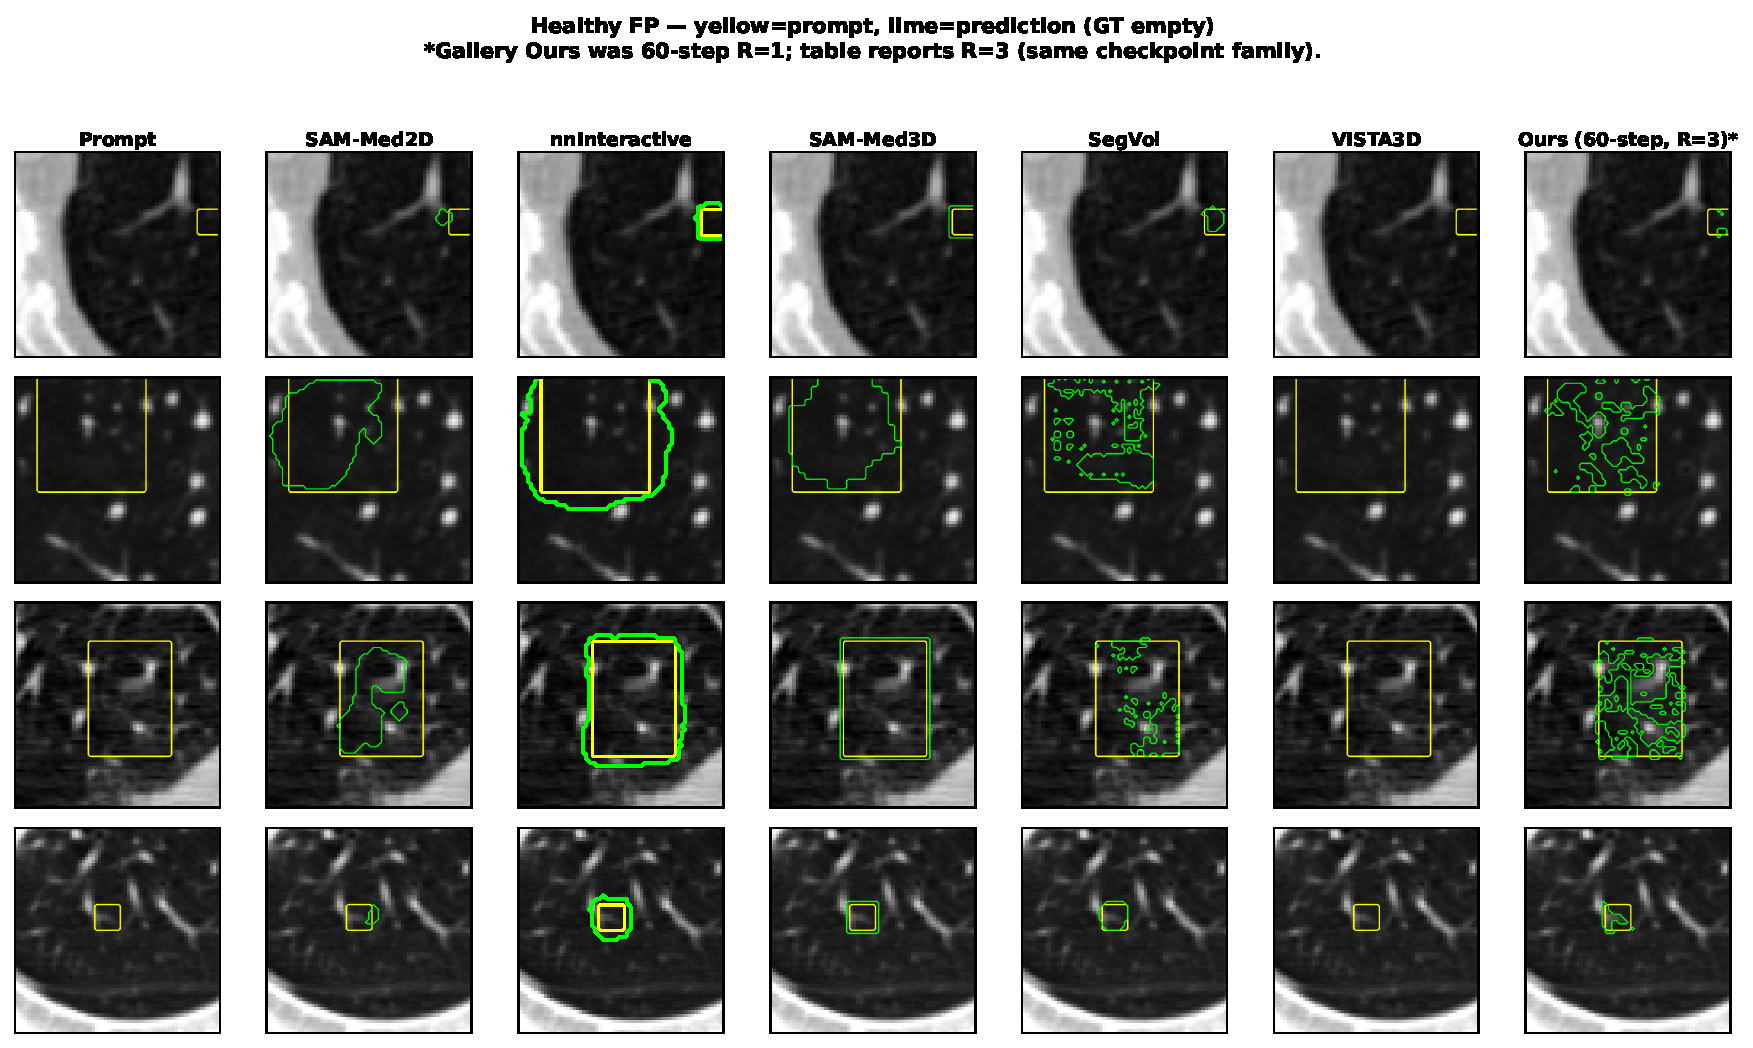
\includegraphics[width=\textwidth]{figures/fig_qual_healthy_fp.pdf}
  \caption{Healthy false-positive probe: random boxes in nodule-free
  lung (yellow~=~prompt contour, green~=~predicted mask fill; GT empty).
  Columns match Figure~\ref{fig:qual-lidc} in the main paper.
  Object-centric baselines often fill the box; Ours
  (\(60\)-step, \(R{=}3\); Table~\ref{tab:healthy_fp} in the main paper)
  is more conservative.}
  \label{fig:qual-fp}
\end{figure*}

\begin{figure*}[t]
  \centering
  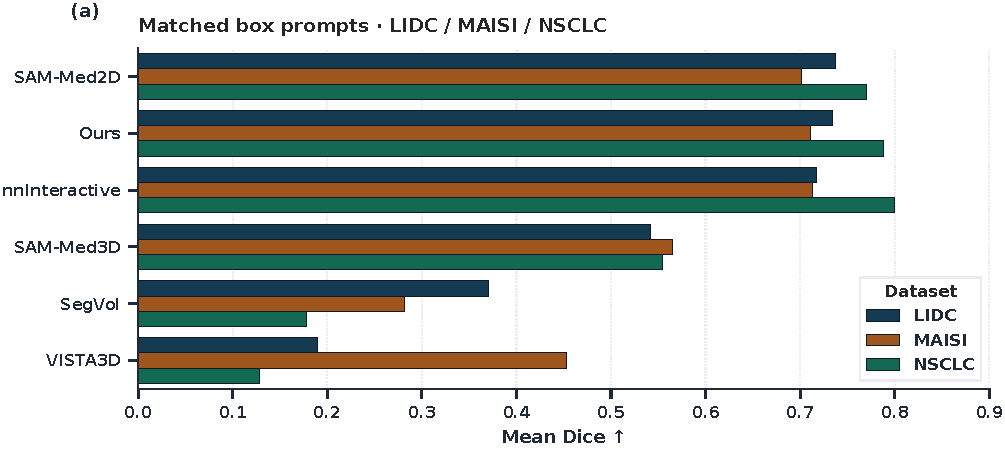
\includegraphics[width=\textwidth]{figures/fig_benchmark_dice_3datasets.pdf}
  \caption{Mean Dice under matched box prompts on LIDC, MAISI, and
  NSCLC (grouped by method). Hatched bars highlight Ours.
  Aggregate numbers match Table~\ref{tab:cross} in the main paper.}
  \label{fig:bench}
\end{figure*}

\begin{figure}[t]
  \centering
  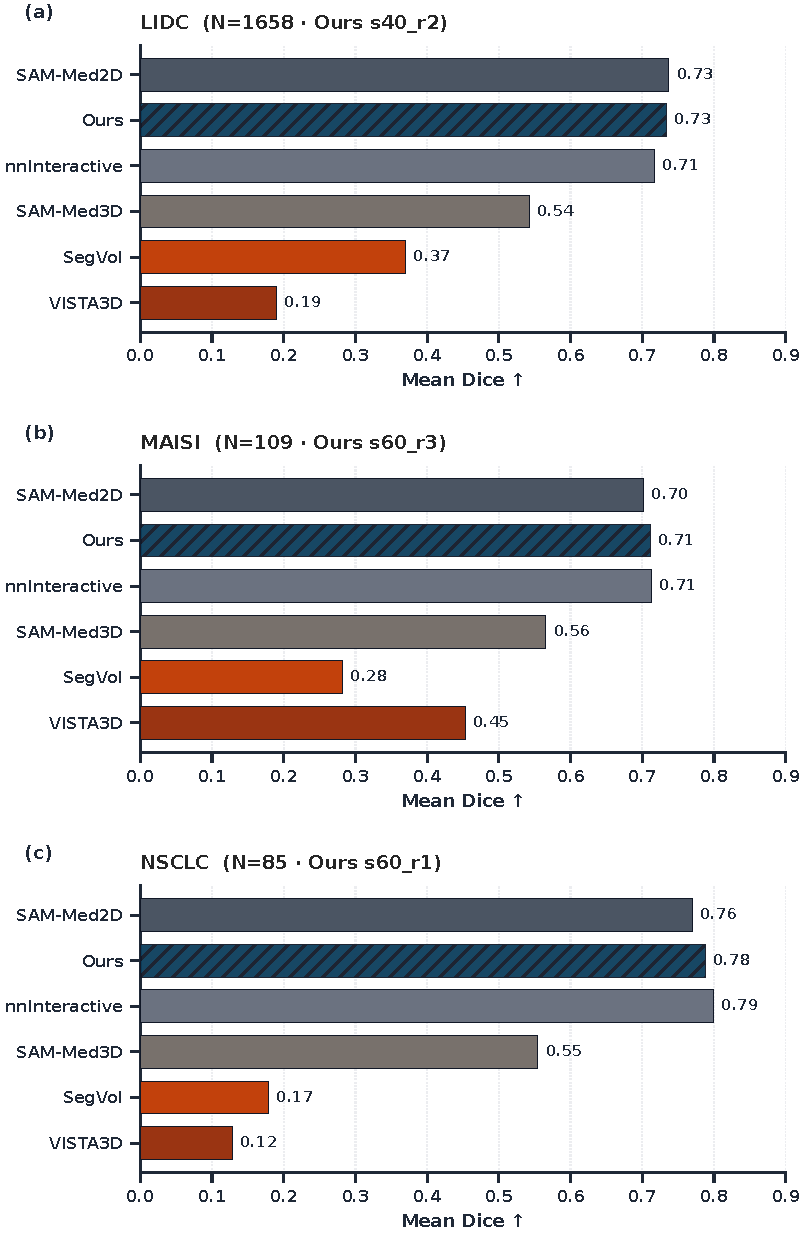
\includegraphics[width=\linewidth]{figures/fig_benchmark_dice_per_dataset.pdf}
  \caption{Per-dataset Dice under the same matched box prompts
  (LIDC, MAISI, NSCLC). Ours uses dataset-specific RF configs.}
  \label{fig:bench-per}
\end{figure}

\begin{figure*}[t]
  \centering
  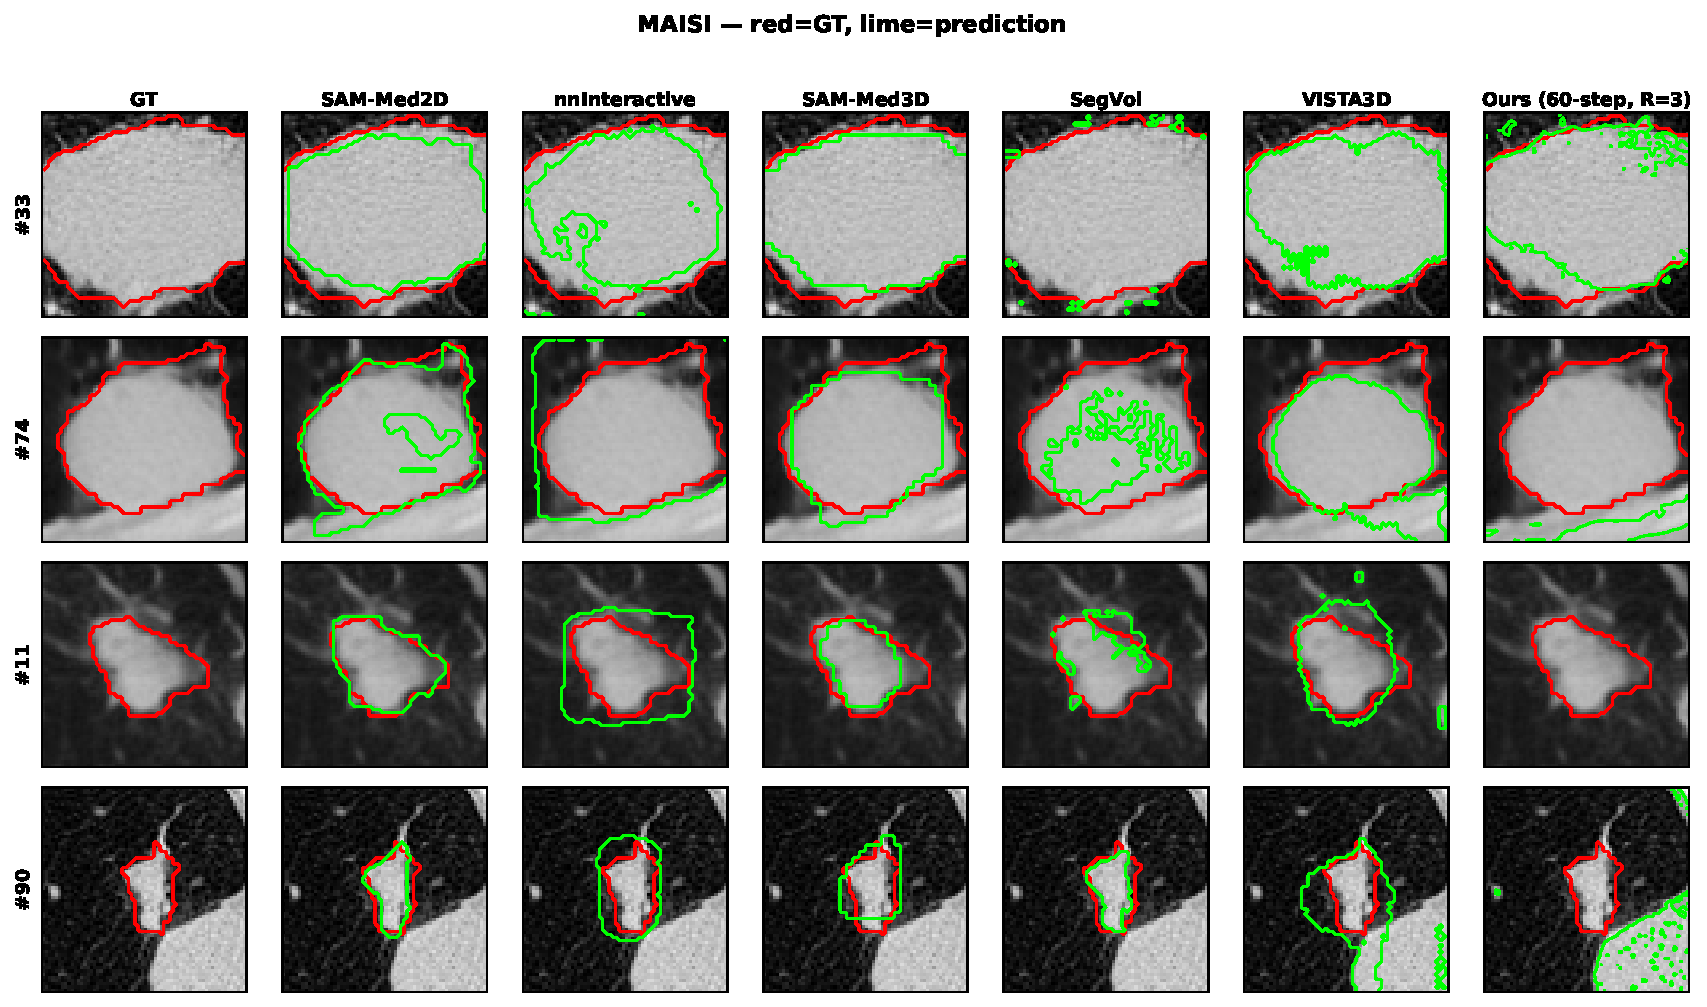
\includegraphics[width=\textwidth]{figures/fig_qual_maisi.pdf}\\[0.12em]
  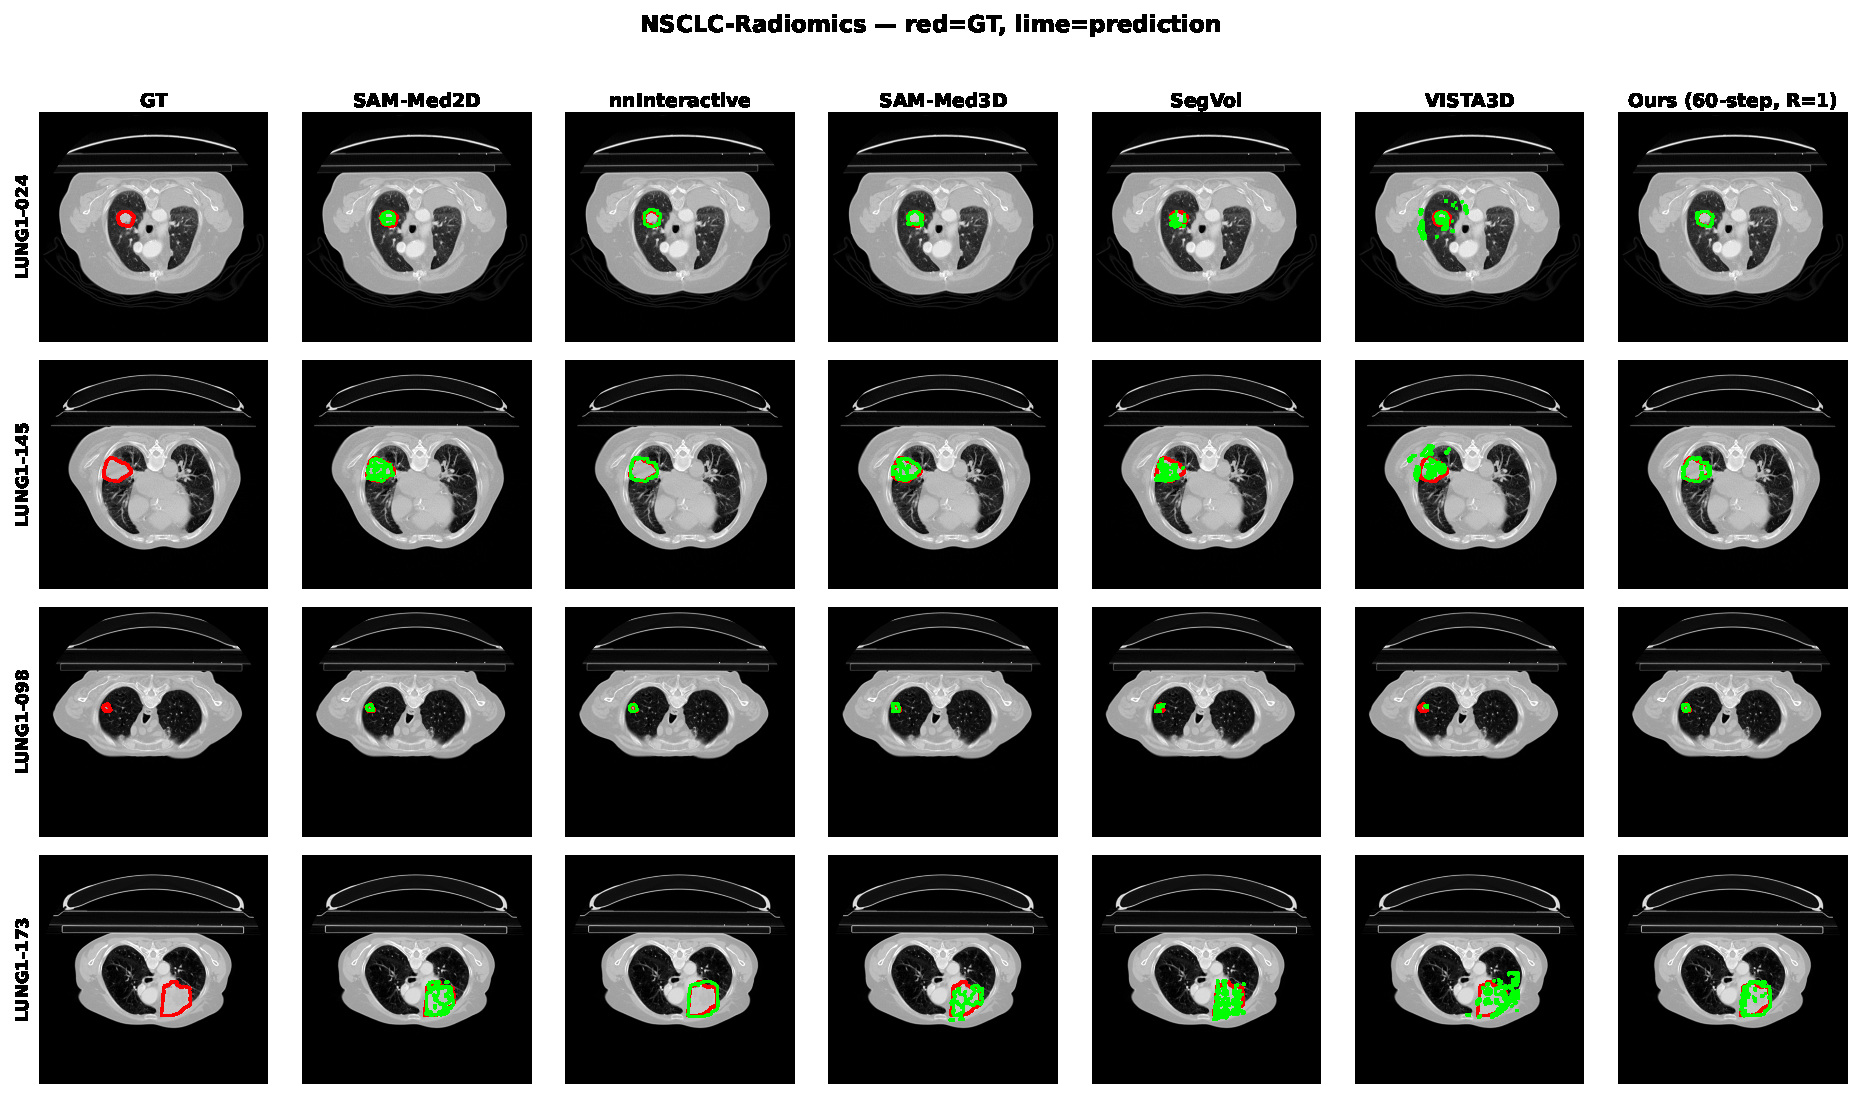
\includegraphics[width=\textwidth]{figures/fig_qual_nsclc.pdf}
  \caption{Cross-dataset qualitative overlays (red~=~GT, lime~=~prediction).
  Columns: GT, SAM-Med2D, nnInteractive, SAM-Med3D, SegVol, VISTA3D, Ours.
  Top: MAISI synthetic nodules (Ours \(60\)-step, \(R{=}3\)).
  Bottom: NSCLC-Radiomics \(64^3\) tumor patches (Ours \(60\)-step, \(R{=}1\);
  cases LUNG1-024 / 145 / 098 / 173).
  Illustrative examples under matched boxes; see Table~\ref{tab:cross}
  in the main paper for aggregate Dice.}
  \label{fig:qual-cross}
\end{figure*}

\begin{figure*}[t]
  \centering
  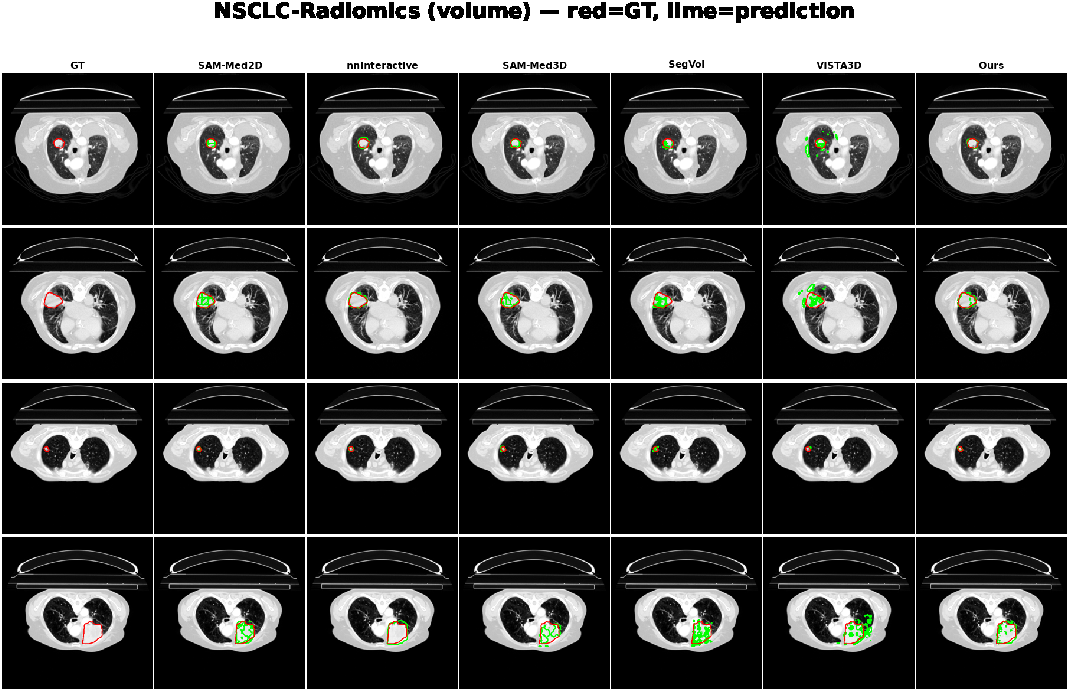
\includegraphics[width=\textwidth]{figures/fig_qual_nsclc_volume.pdf}
  \caption{NSCLC-Radiomics whole-volume overlays for the same four
  patients as in Figure~\ref{fig:qual-cross} (red~=~GT,
  lime~=~prediction; Ours \(60\)-step, \(R{=}1\)). Patch crops in
  Figure~\ref{fig:qual-cross} use the matched \(64^3\) regions from
  these volumes.}
  \label{fig:qual-nsclc-vol}
\end{figure*}
\FloatBarrier

% ----------------------------------------------------------------------
\section{Ablation: Steps and Refine Rounds}
\label{sec:supp:ablation}
% ----------------------------------------------------------------------
Table~\ref{tab:ablation} and Figures~\ref{fig:ablation}
and~\ref{fig:qual-ablation} are Table~S2 and Figures~S6--S7 in the
main paper. They vary inference steps and refine rounds \(R\)
on the LIDC positive set (same checkpoint). Moderate compute
(\(40\) steps, \(R{=}2\)) is sufficient for near-peak Dice; several
\(R{=}3\) settings underperform the main \(R{=}2\) operating point, and
\(80\)-step/\(R{=}2\) also does not beat it.
Figure~\ref{fig:qual-ablation} shows the corresponding overlays: coarse
\(30\)-step residuals clean up by \(40\)-step/\(R{=}2\), after which
contours stay visually stable---consistent with the flat Dice curve.

\begin{table}[t]
\centering
\caption{Ablation of inference steps and refine rounds on LIDC
positive test (\(N{=}1658\)).}
\label{tab:ablation}
\begin{tabular}{lcc}
\toprule
Configuration & Dice \(\uparrow\) & IoU \(\uparrow\) \\
\midrule
30-step, \(R{=}3\) & 0.72 & 0.58 \\
40-step, \(R{=}3\) & 0.72 & 0.59 \\
\textbf{40-step, \(R{=}2\)} & \textbf{0.73} & \textbf{0.59} \\
60-step, \(R{=}3\) & 0.72 & 0.58 \\
80-step, \(R{=}2\) & 0.72 & 0.59 \\
\bottomrule
\end{tabular}
\end{table}

\begin{figure}[t]
  \centering
  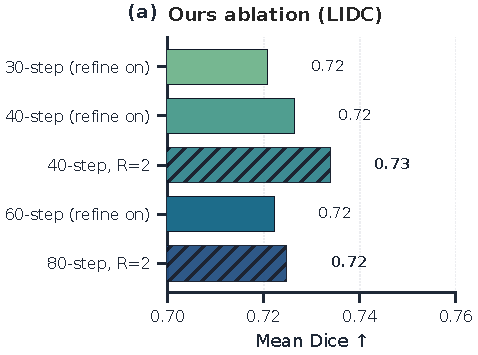
\includegraphics[width=\linewidth]{figures/fig_ablation_steps.pdf}
  \caption{Ablation of RF inference steps and refine rounds on LIDC
  positives. The hatched bar is the main reported config
  (\(40\)-step, \(R{=}2\)).}
  \label{fig:ablation}
\end{figure}

\begin{figure*}[t]
  \centering
  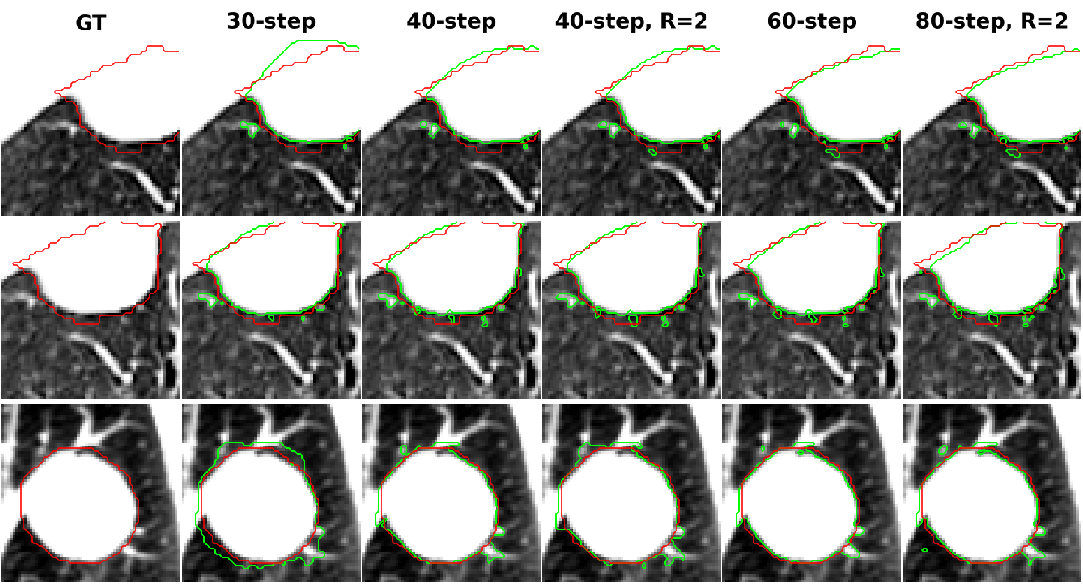
\includegraphics[width=\textwidth]{figures/fig_qual_ablation.pdf}
  \caption{Ablation qualitative overlays on LIDC (red~=~GT,
  lime~=~prediction) for the step/\(R\) settings in
  Table~\ref{tab:ablation}. Contours tighten from \(30\)-step to the
  main \(40\)-step/\(R{=}2\) config and then remain stable.}
  \label{fig:qual-ablation}
\end{figure*}
\FloatBarrier

% ----------------------------------------------------------------------
\section{Cross-Dataset Healthy False-Positive Probe}
\label{sec:supp:healthy-fp-cross}
% ----------------------------------------------------------------------
We repeat the LIDC healthy false-positive protocol
(Table~\ref{tab:healthy_fp} in the main paper) on nodule-free MAISI
and NSCLC patches: random lung boxes (same size prior and seed),
empty GT, and mean predicted mask volume (mm\(^3\)).
Table~\ref{tab:healthy-fp-cross} reports aggregate volumes;
Figures~\ref{fig:fp-tradeoff-maisi}--\ref{fig:fp-tradeoff-nsclc}
show the volume bars and true-nodule Dice vs.\ FP-volume trade-offs;
Figures~\ref{fig:qual-fp-maisi}--\ref{fig:qual-fp-nsclc} give
qualitative overlays (yellow~=~prompt box, lime~=~prediction).
Ours uses the same dataset-specific RF settings as
Table~\ref{tab:cross} in the main paper
(MAISI: \(60\)-step, \(R{=}3\); NSCLC: \(60\)-step, \(R{=}1\)).
Across both sets, Ours remains the lowest-\emph{non-silent} volume among
methods that stay competitive on true nodules; VISTA3D is silent
(\(0\,\mathrm{mm}^3\)) but weak on positive Dice
(Table~\ref{tab:cross} in the main paper). SAM-Med3D returns an empty
mask on \(\sim\)1\% of prompts (same rate as LIDC); those rows are
present with zero volume rather than missing.

\begin{table*}[t]
\centering
\caption{Healthy false-positive probe on MAISI (\(N{=}2848\)) and
NSCLC (\(N{=}2720\)) nodule-free patches: mean predicted volume
(mm\(^3\)). Lowest non-silent volume per column in \textbf{bold}.
Dice against empty GT is omitted.}
\label{tab:healthy-fp-cross}
\begin{tabular}{lcc}
\toprule
Method & MAISI vol.\ (mm\(^3\)) \(\downarrow\) &
NSCLC vol.\ (mm\(^3\)) \(\downarrow\) \\
\midrule
VISTA3D$^\dagger$
  & \(0\) & \(0\) \\
\textbf{Ours}
  & \textbf{958} & \textbf{1405} \\
SegVol
  & 1567 & 1583 \\
SAM-Med2D
  & 2016 & 1965 \\
SAM-Med3D
  & 2780 & 2972 \\
nnInteractive
  & 4168 & 4102 \\
\bottomrule
\end{tabular}\\[0.25em]
{\footnotesize $^\dagger$Near-silent on healthy prompts (cf.\
Table~\ref{tab:cross} in the main paper for true-nodule Dice).
Ours: MAISI \(60\)-step/\(R{=}3\); NSCLC \(60\)-step/\(R{=}1\).}
\end{table*}

\begin{figure*}[t]
  \centering
  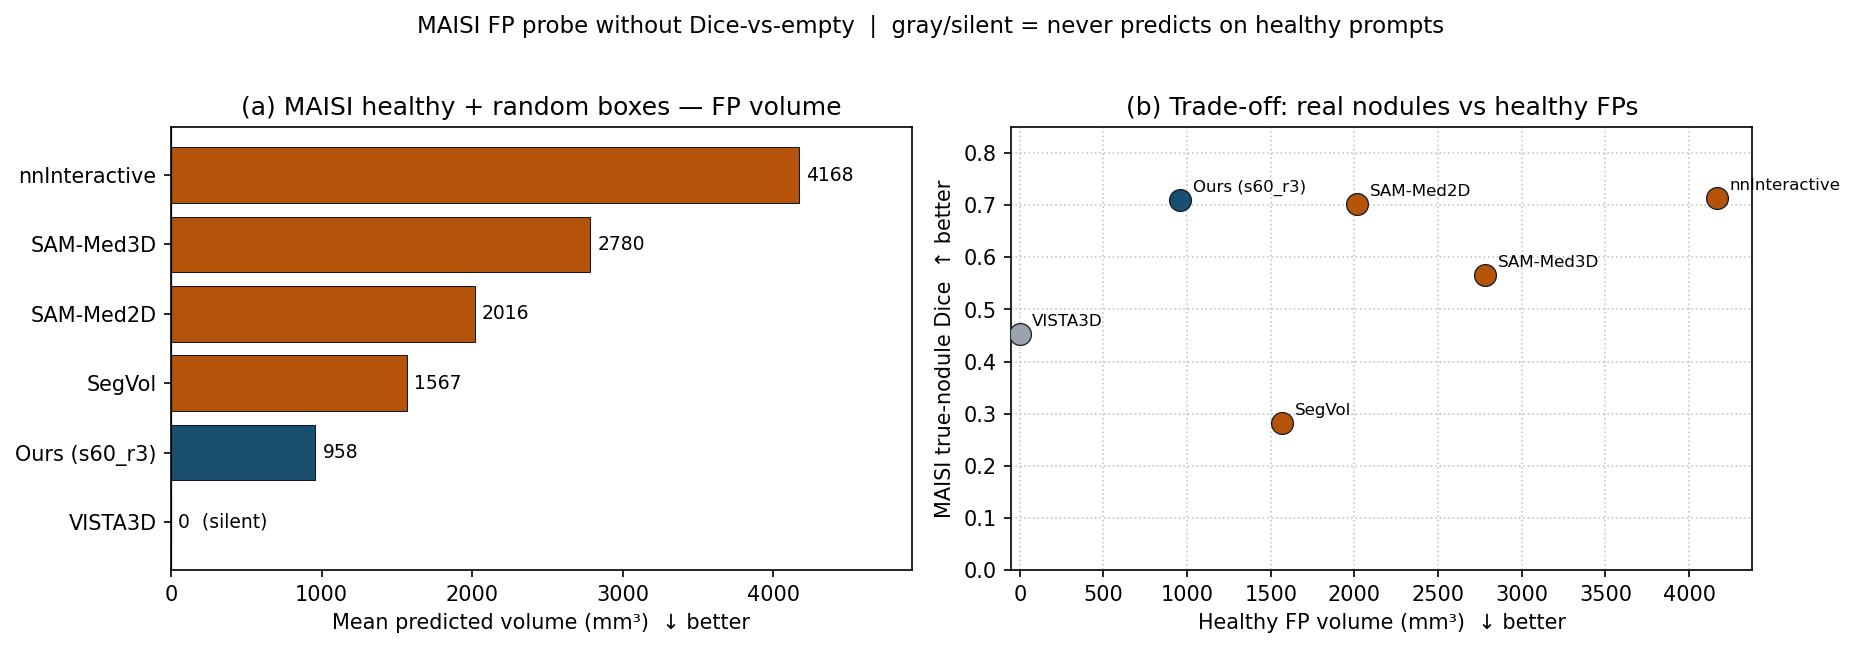
\includegraphics[width=\textwidth]{figures/fig_healthy_fp_tradeoff_maisi.pdf}
  \caption{Healthy FP probe on MAISI:
  (a)~mean predicted volume under random empty-GT boxes;
  (b)~MAISI true-nodule Dice vs.\ healthy FP volume.
  Silent models (e.g., VISTA3D) sit at zero volume but low positive Dice
  (Table~\ref{tab:cross} in the main paper).}
  \label{fig:fp-tradeoff-maisi}
\end{figure*}

\begin{figure*}[t]
  \centering
  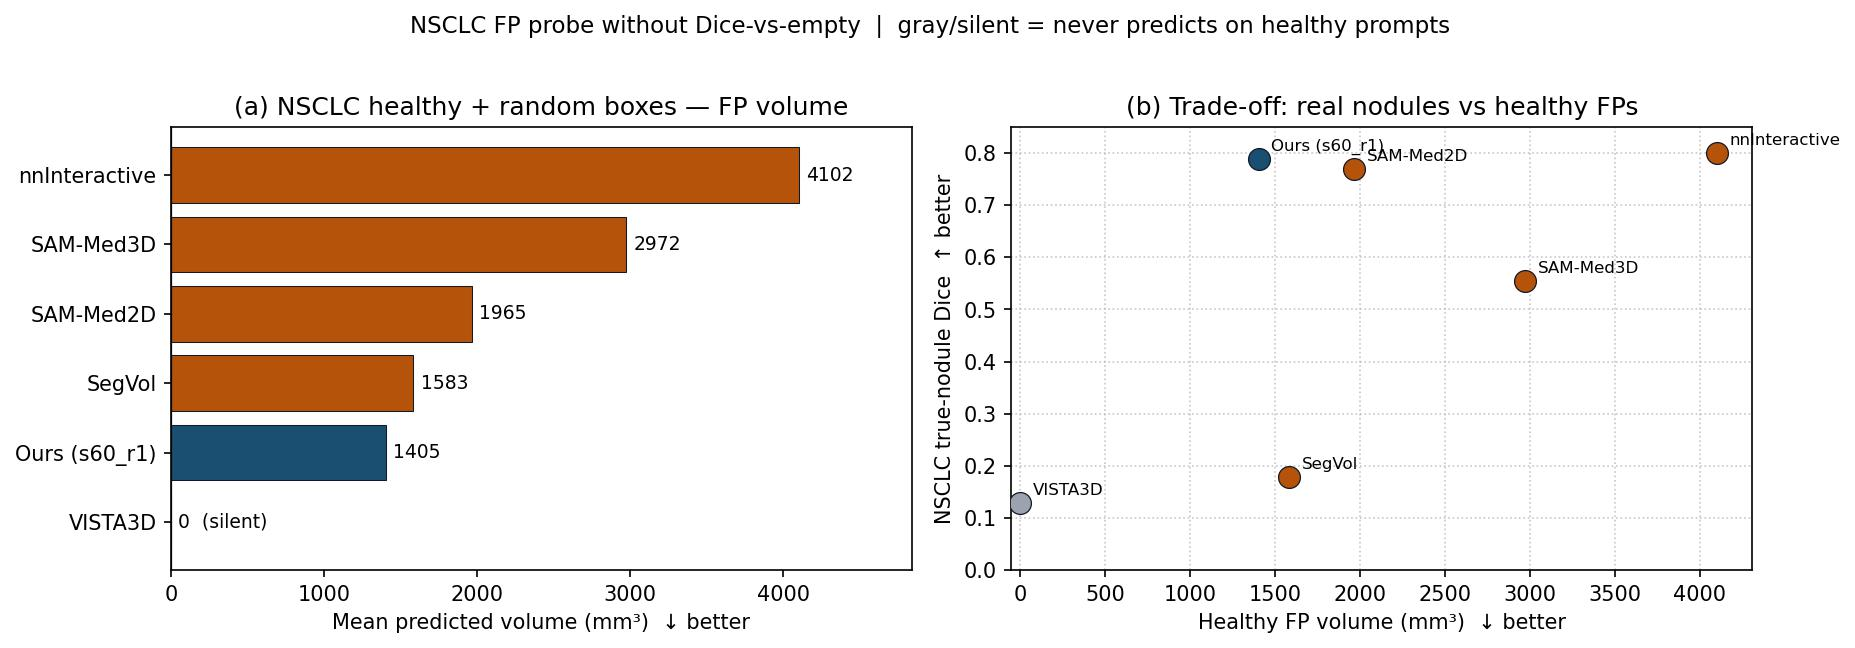
\includegraphics[width=\textwidth]{figures/fig_healthy_fp_tradeoff_nsclc.pdf}
  \caption{Healthy FP probe on NSCLC under the same protocol as
  Figure~\ref{fig:fp-tradeoff-maisi}
  (Ours \(60\)-step, \(R{=}1\); Table~\ref{tab:healthy-fp-cross}).}
  \label{fig:fp-tradeoff-nsclc}
\end{figure*}

\begin{figure*}[t]
  \centering
  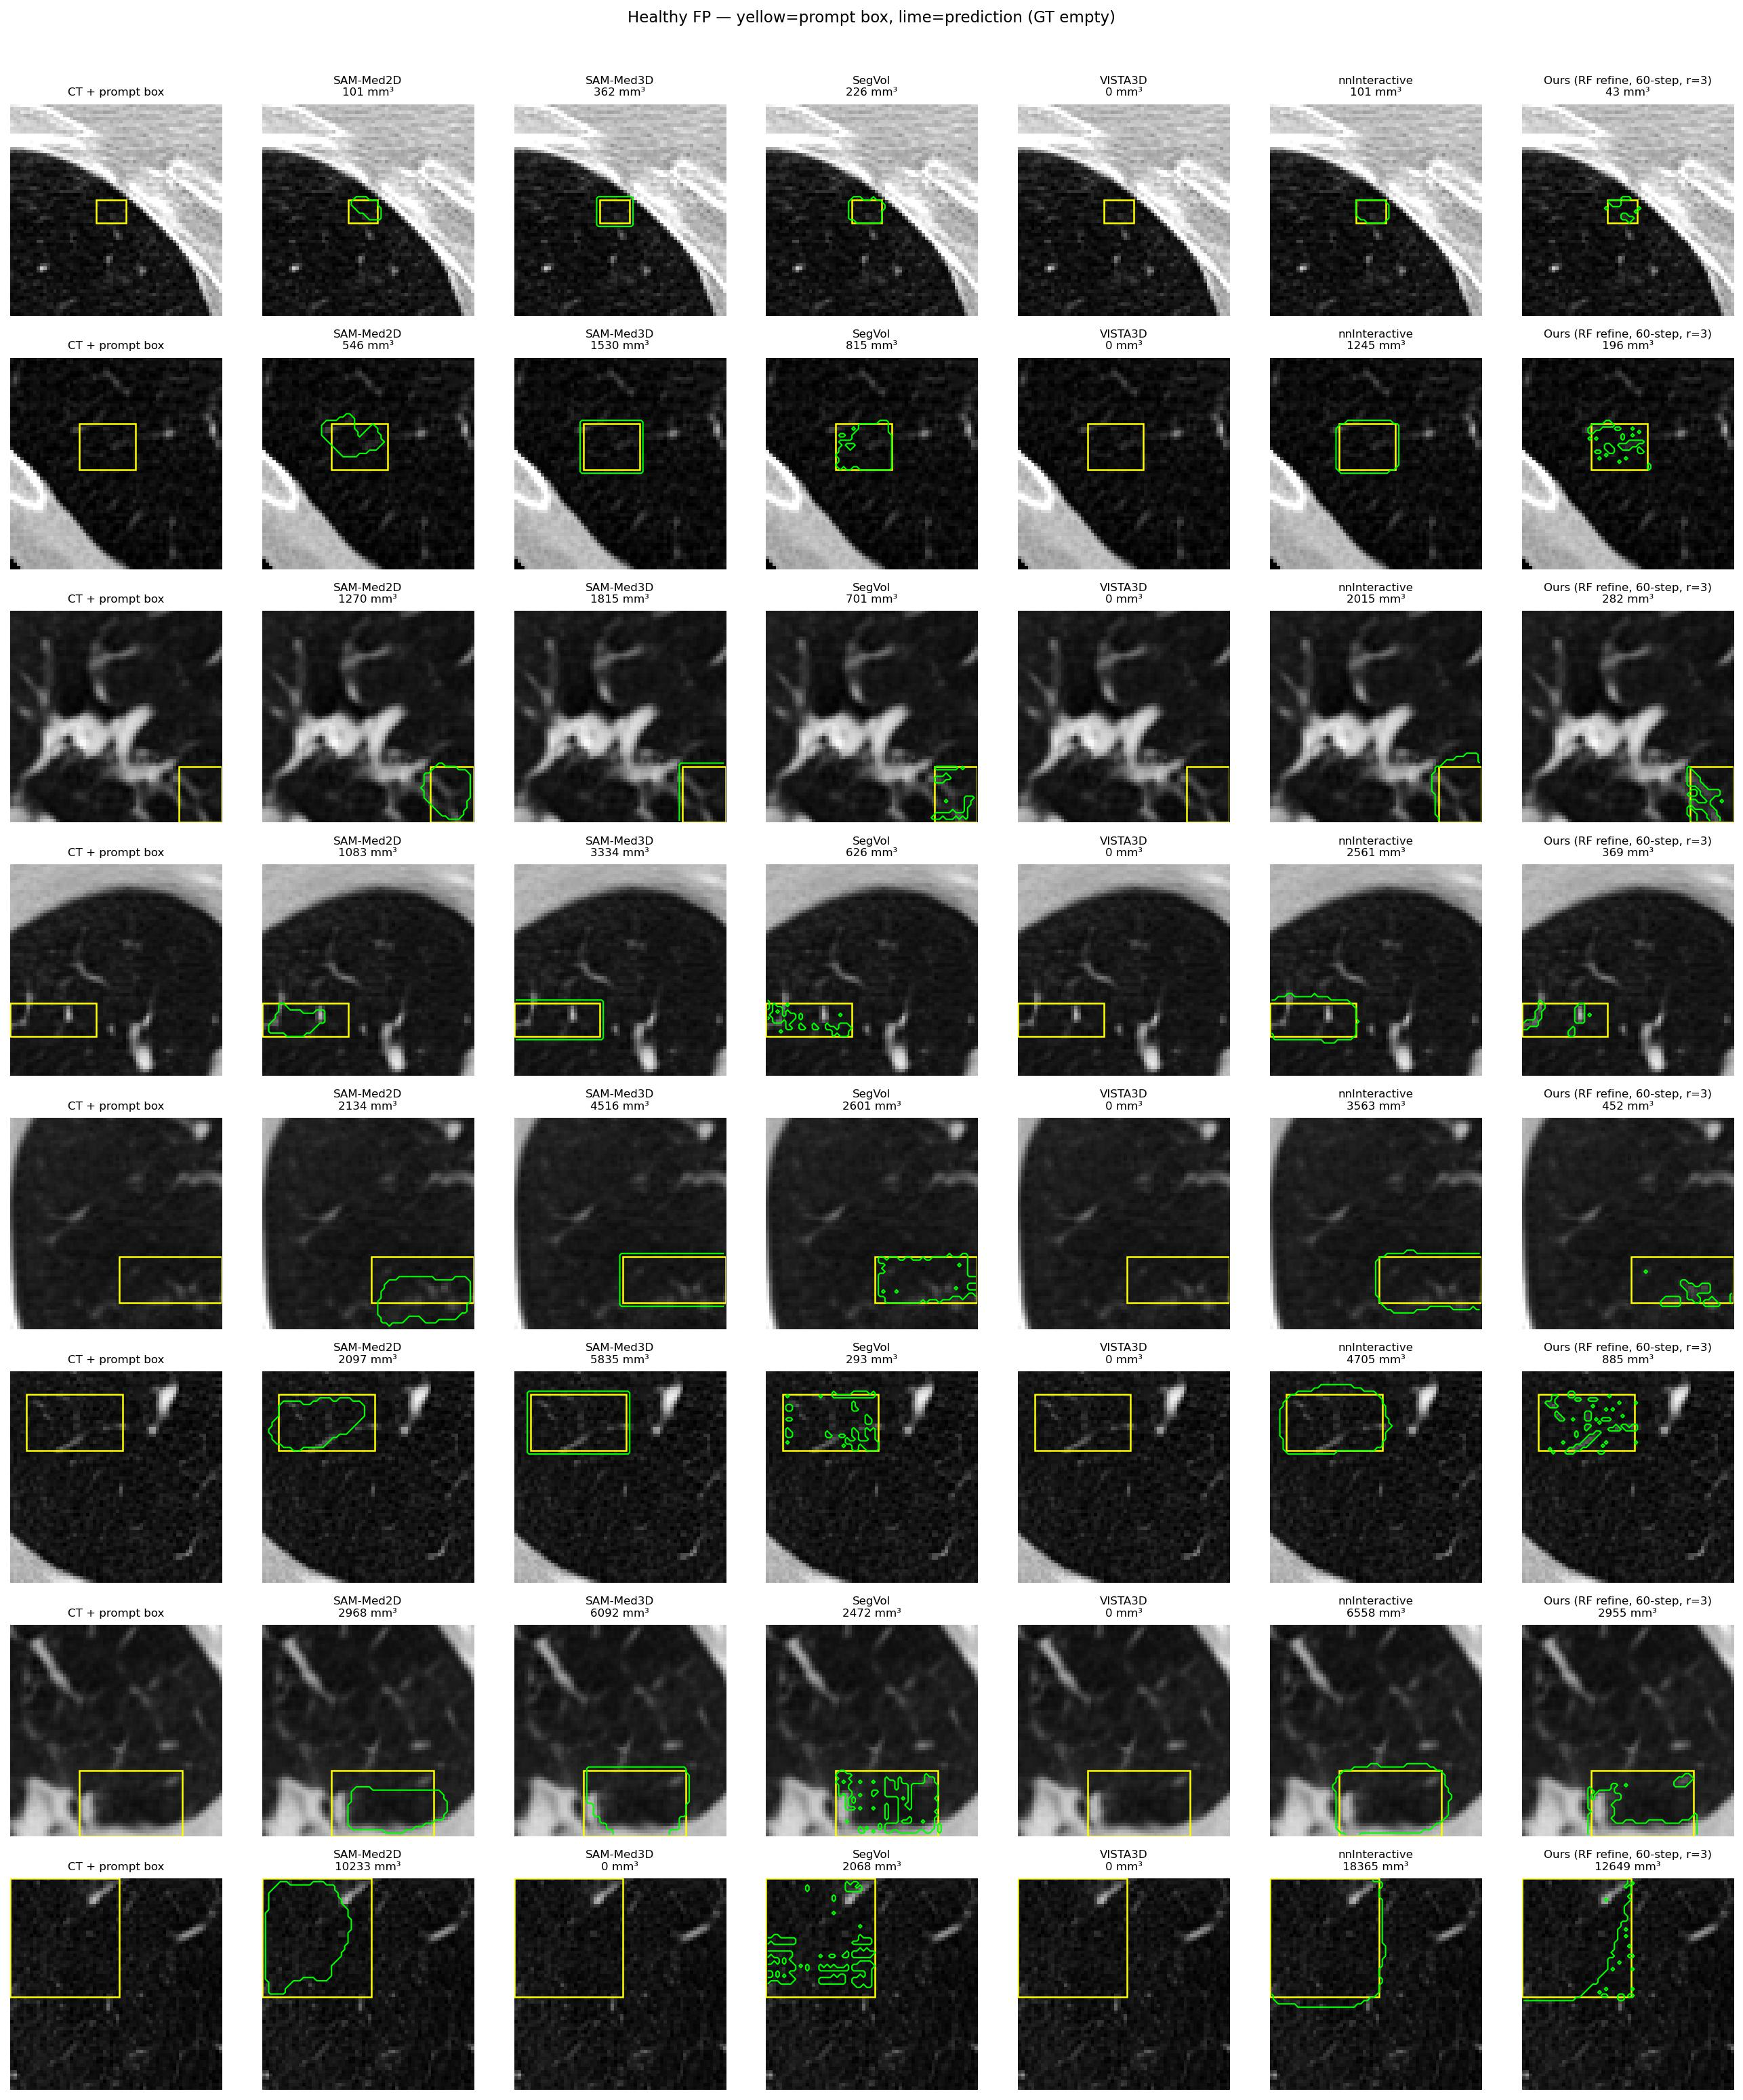
\includegraphics[width=\textwidth]{figures/fig_qual_healthy_fp_maisi.pdf}
  \caption{MAISI healthy false-positive probe: random boxes in
  nodule-free patches (yellow~=~prompt, lime~=~prediction; GT empty).
  Columns: CT+box, SAM-Med2D, SAM-Med3D, SegVol, VISTA3D, nnInteractive,
  Ours (\(60\)-step, \(R{=}3\)). Object-centric baselines often fill the
  box; Ours is more conservative (Table~\ref{tab:healthy-fp-cross}).}
  \label{fig:qual-fp-maisi}
\end{figure*}

\begin{figure*}[t]
  \centering
  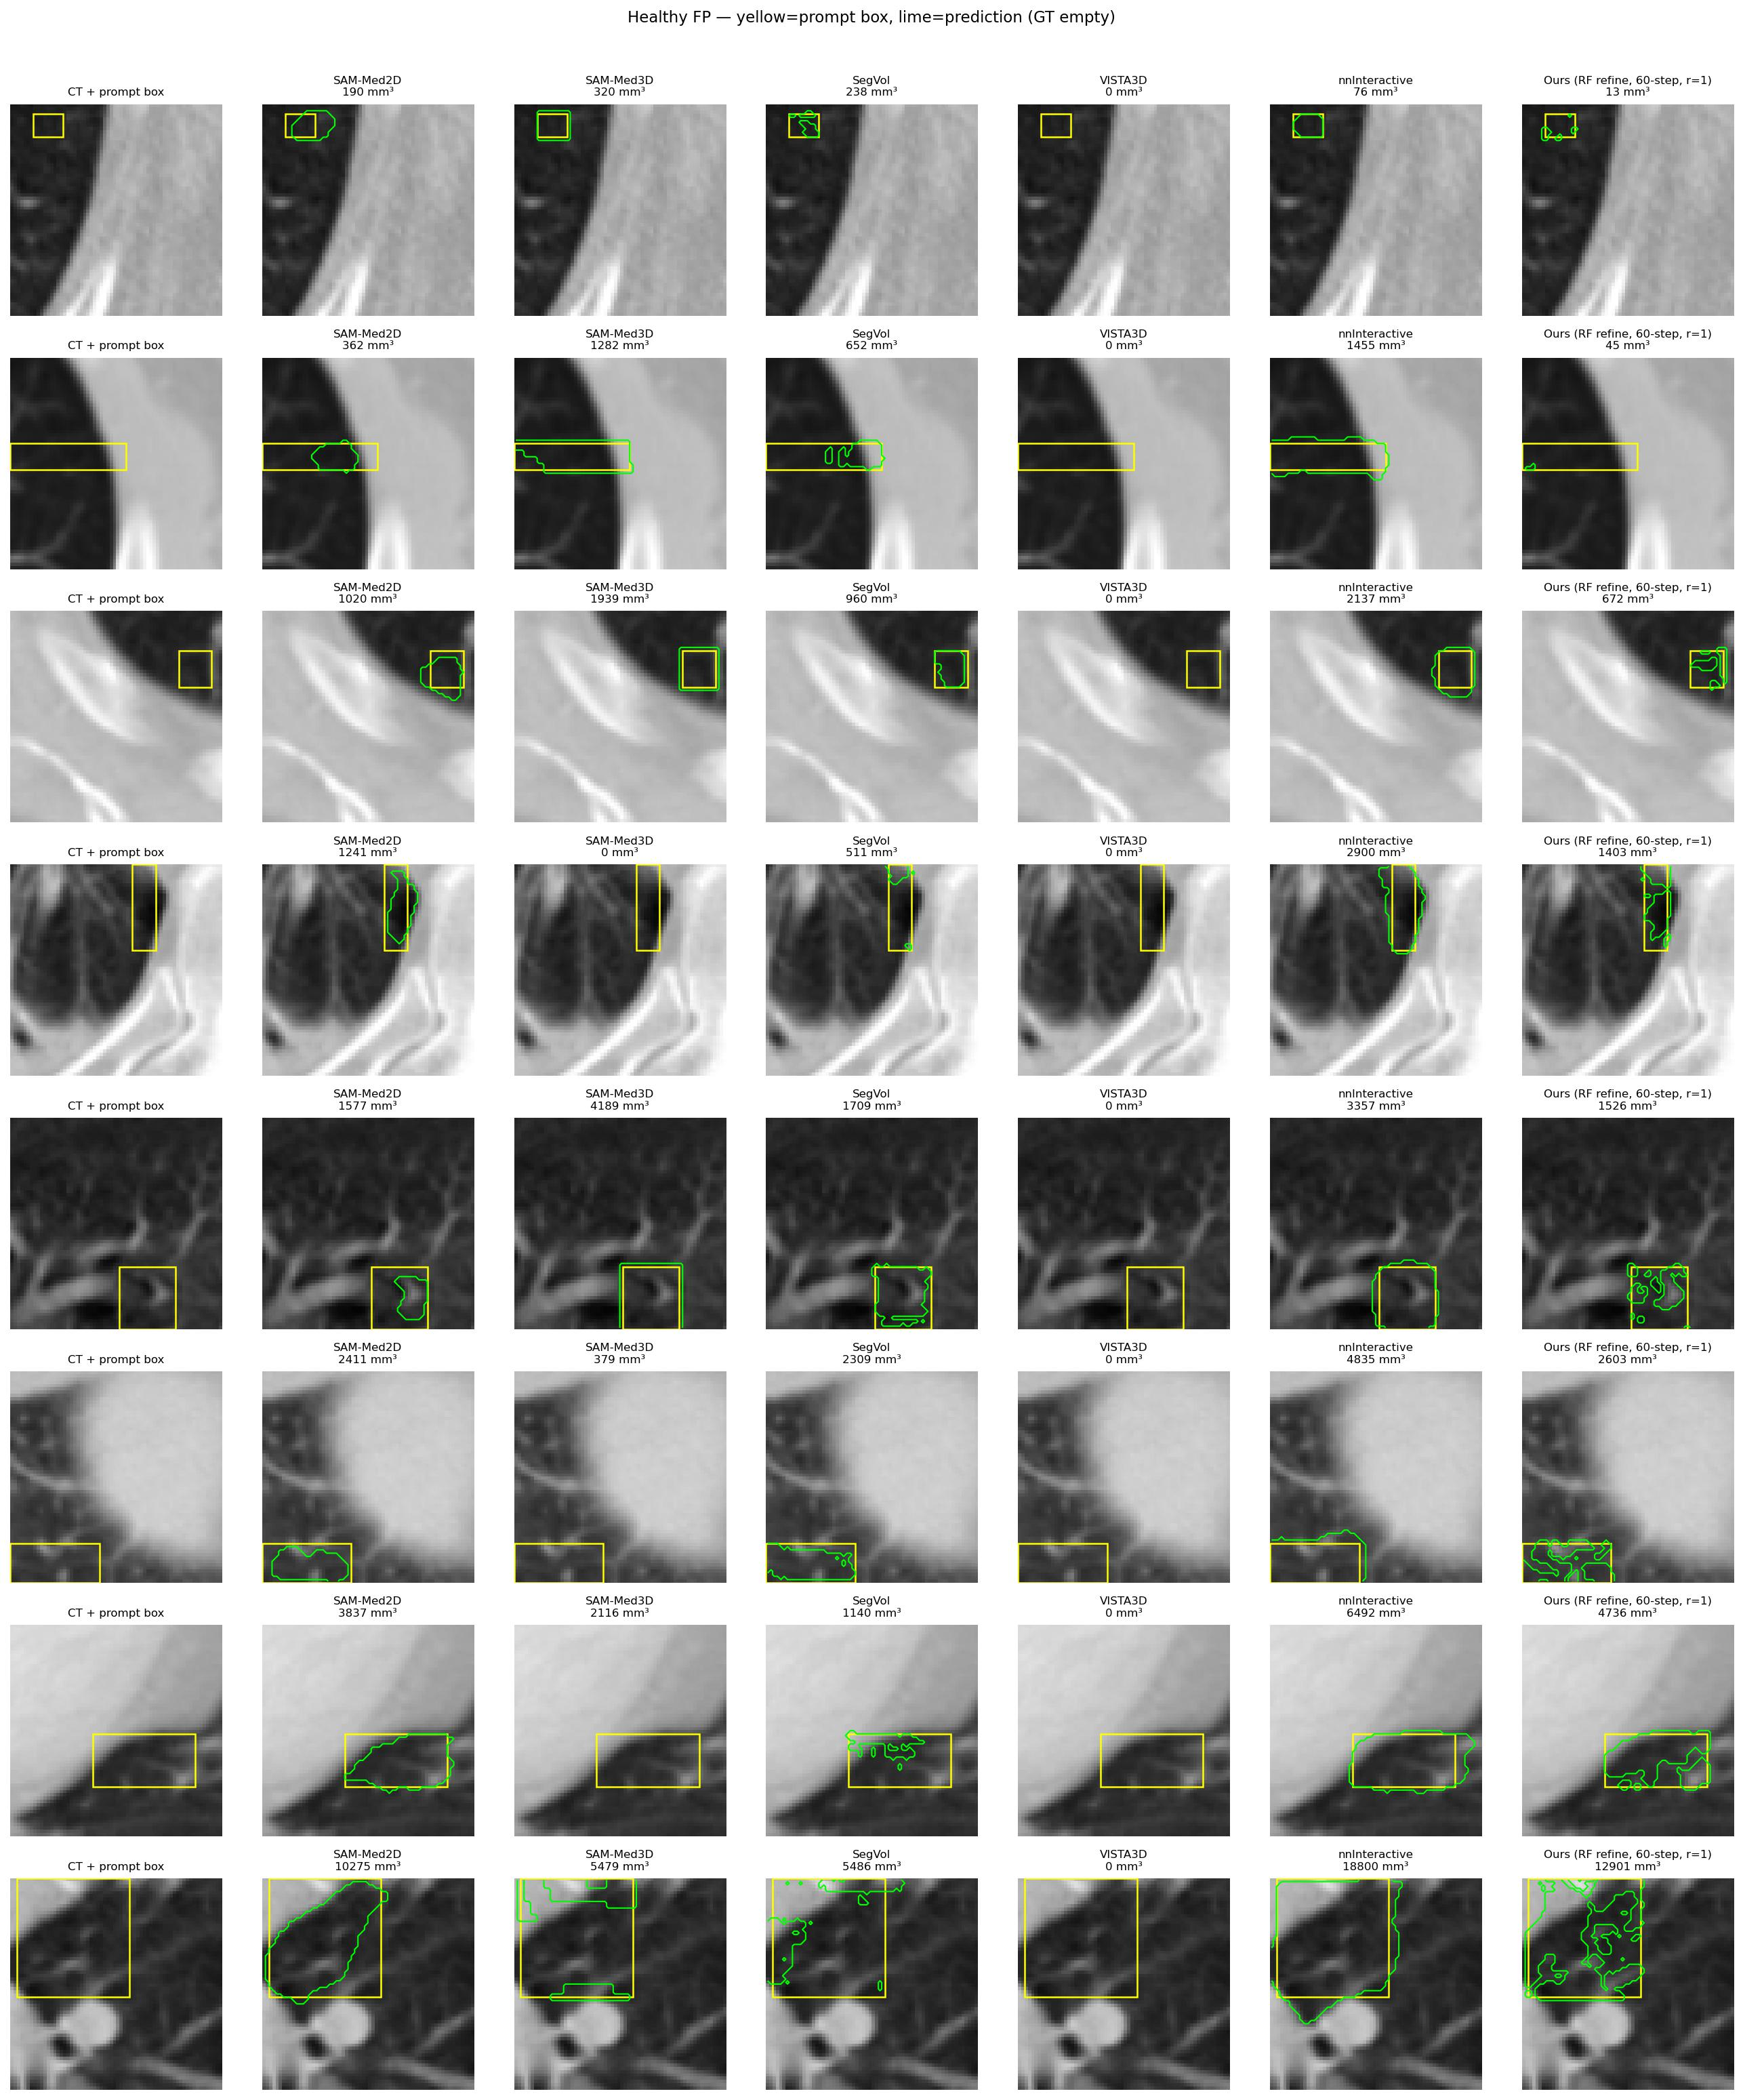
\includegraphics[width=\textwidth]{figures/fig_qual_healthy_fp_nsclc.pdf}
  \caption{NSCLC healthy false-positive probe under the same protocol
  (Ours \(60\)-step, \(R{=}1\)). Layout matches
  Figure~\ref{fig:qual-fp-maisi}; see Table~\ref{tab:healthy-fp-cross}.}
  \label{fig:qual-fp-nsclc}
\end{figure*}

\end{document}
